
\chapter{Actual Outcomes}

\pagenumbering{arabic}
\setcounter{page}{38}

% losses highlight 

\section{GAN losses (200 epochs)}

\begin{table}[h]
    \centering
    \begin{tabular}{|l|l|} \hline 
        Discriminator\_A & 0.083 \\ \hline 
        Generator\_A & 0.613 \\ \hline 
        Cycle\_A & 0.298 \\ \hline 
        Identity\_A & 0.141 \\ \hline 
        Discriminator\_B & 0.000 \\ \hline 
        Generator\_B & 1.000 \\ \hline 
        Cycle\_B & 0.299 \\ \hline 
        Identity\_B & 0.032 \\ \hline
        
    \end{tabular}
    
    \caption{Losses on training for 200 epochs}
    \label{table:table_loss}
   
   \noindent where,\\
    A = Black and White Dataset\\
    B= Colored Dataset \\
\end{table}
     
\noindent The losses for Generators and Discriminators reached the values as in \ref{table:table_loss} at the end of 200th epoch. The discriminator for colored image had its loss converged to 0 while the loss of the generator peaked to 1.  The effect of adversarial nature of the networks was seen in the graph of losses. Color generator and color discriminator losses reached plateau at around 160 epochs.

\clearpage
\section{Test Results (different sized inputs)}
% test results


\begin{figure}[h!]
  \centering
  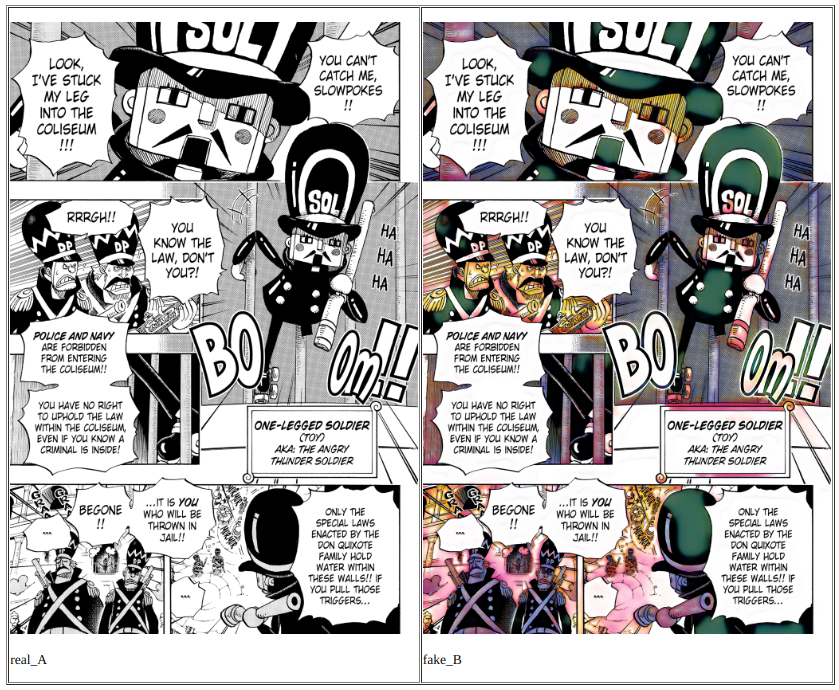
\includegraphics[width=0.8\textwidth]{chapter/actual/acx.png}
 
  \label{fig:final UI}
\end{figure}
\begin{figure}[h!]
  \centering
  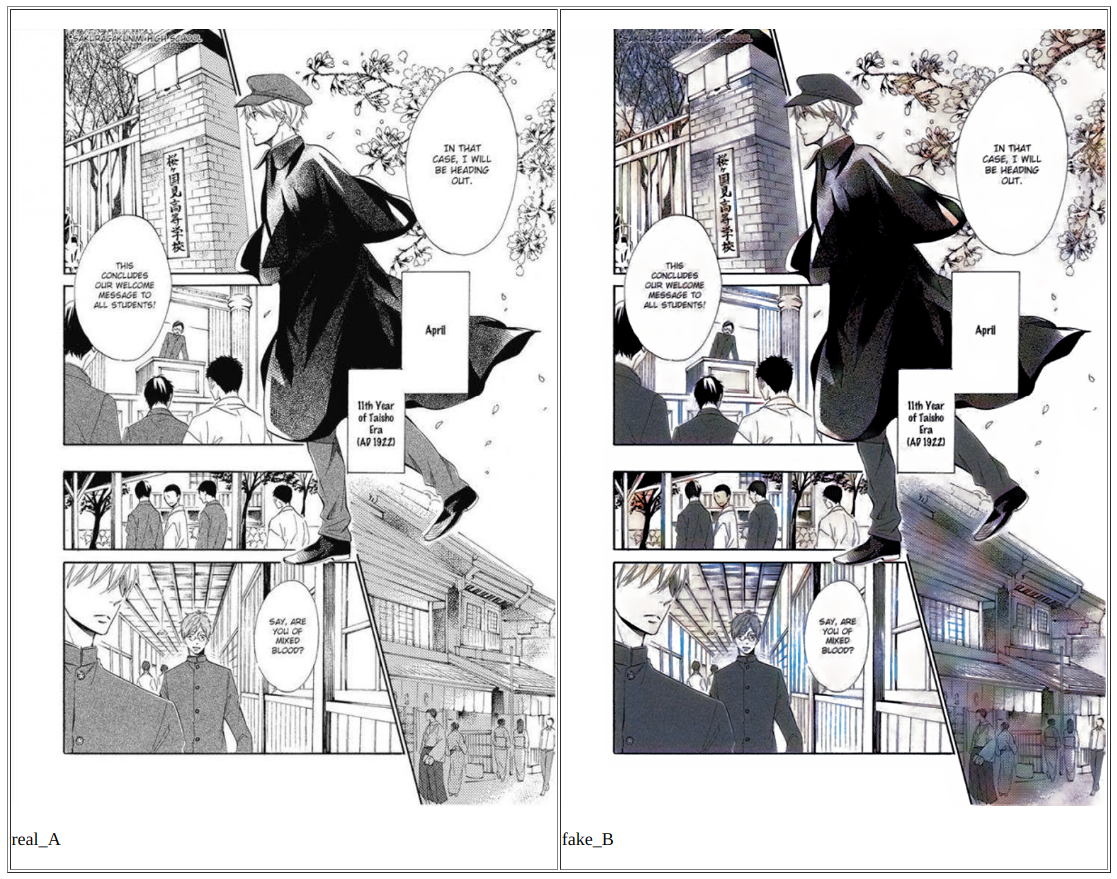
\includegraphics[width=0.8\textwidth]{chapter/actual/acu.png}
  \label{fig:final UI}
\end{figure}
\newpage
\begin{figure}[h!]
  \centering
  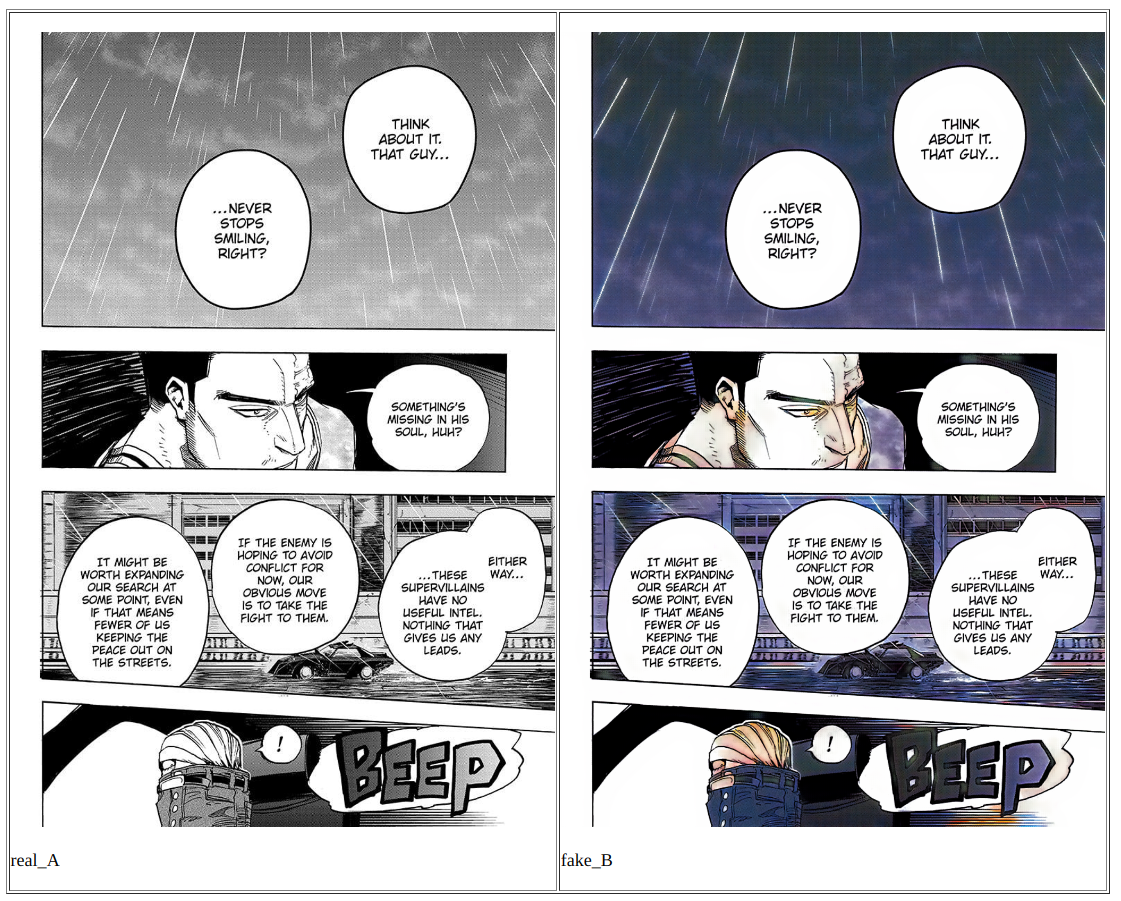
\includegraphics[width=0.8\textwidth]{chapter/actual/acy.png}
  \label{fig:final UI}
\end{figure}
\begin{figure}[h!]
  \centering
  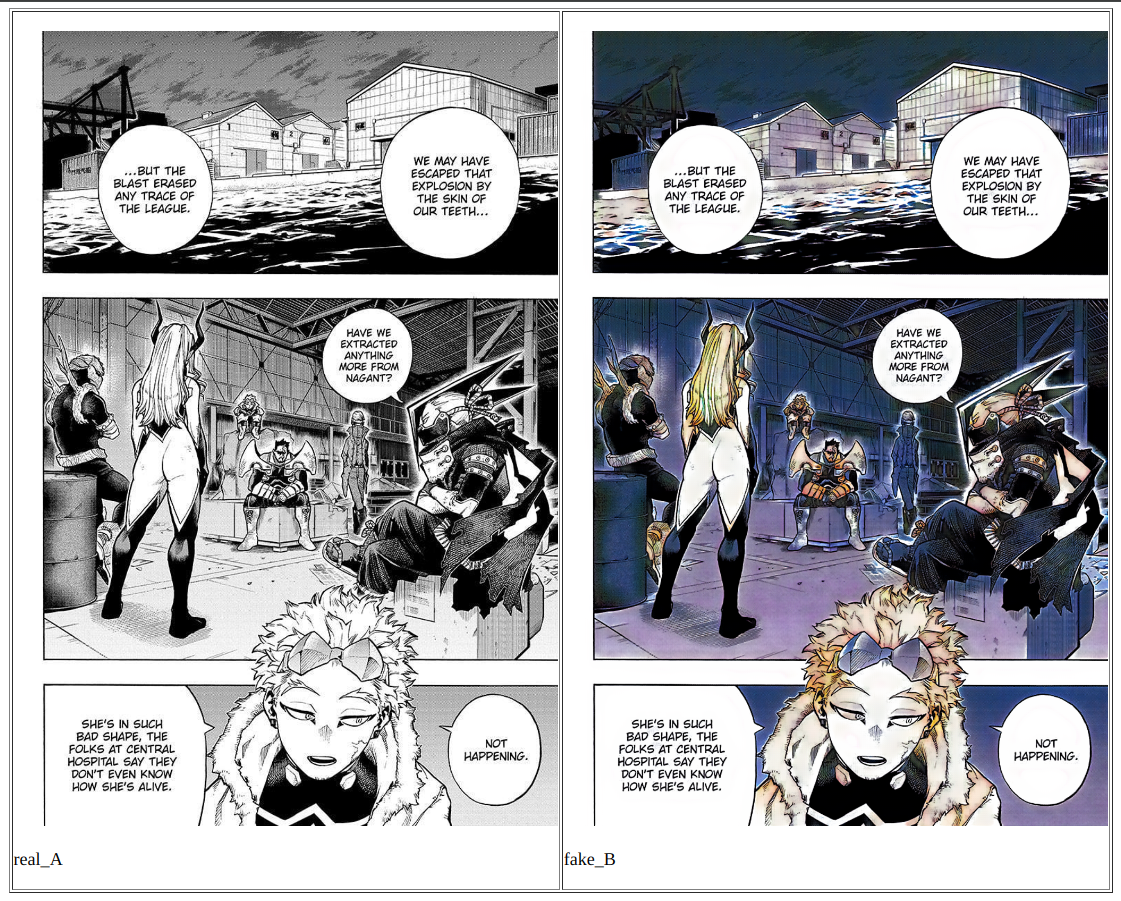
\includegraphics[width=0.8\textwidth]{chapter/actual/acz.png}
  \label{fig:final UI}
\end{figure}

For testing and deployment, we only need to load the color generator. So far, it's been impressively consistent with colors across panels on a page, especially in darker and shaded spots where it fills in suitable colors that match the environment's mood. It made sure to steer clear of coloring over text blobs, and inherently white backgrounds.The details in reconstructed image remain intact and the test is well-readable. Despite being trained on cropped images from a small dataset, it's adapting well to a range of new test images. Our model can handle high-definition images of different sizes and colorize them effectively.
% describe kk xa, similar color of hair can be seen, ani text ni high res, text blobs uncolored, any size of input can be given, 256x256 ma train garyo bhane the closer the test input is to 256x256, the better is the op. ani crop garera, resize nagari train garyo bhane, larger test inputs ma better results. 
\clearpage
%limitation
\subsection{Limitations}
While our model excels at coloring manga panels at certain scenarios such as dark room or rainy/cloudy weather, it fails to produce such good results at other scenarios. It also seems to have heavy inclination towards blue color. 

\begin{figure}[hbtp]
    \centering
    \begin{subfigure}[b]{0.48\textwidth}
        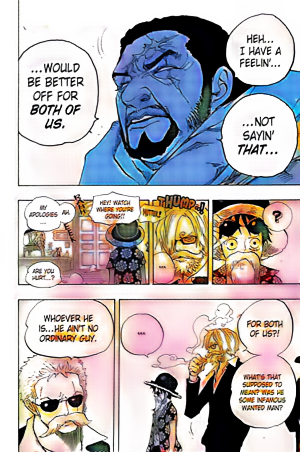
\includegraphics[width=\textwidth]{chapter/actual/ac3.png}
    \end{subfigure}
    \hfill
    \begin{subfigure}[b]{0.45\textwidth}
        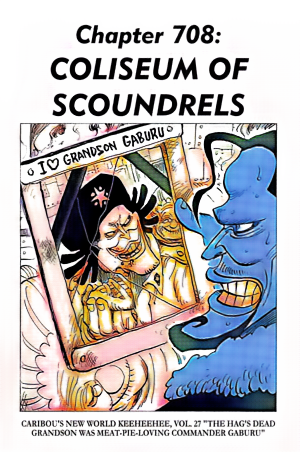
\includegraphics[width=\textwidth]{chapter/actual/ac1.png}
    \end{subfigure}
    \caption{Failed colorized outputs}
        \label{fig:bad_images}
\end{figure}


\section{Performance Evaluation}
% performance evaluation
In evaluating the fidelity of the reconstructed images compared to their original counterparts, we utilized Peak Signal-to-Noise Ratio (PSNR) as a metric. This measure allows for a quantitative evaluation of reconstruction quality, with higher PSNR values indicating higher fidelity. Our assessment involved four different images, each representative of distinct manga panel styles. Across all image pairs, the PSNR values were consistently high, averaging at 24.3742 dB. This average PSNR suggests satisfactory performance of the color generator in reconstructing the images.

To evaluate structural similarity between the original and reconstructed images, we employed the Structural Similarity Index (SSIM). SSIM considers various aspects such as luminance, contrast, and structure, providing a comprehensive assessment. SSIM values range from -1 to 1, with 1 indicating perfect similarity. While slight visual differences were observed between the image pairs, the average SSIM value of 0.9039 confirms that the reconstructed images maintain structural coherence.

In summary, our CycleGAN model has demonstrated reasonable performance based on both PSNR and SSIM scores, indicating successful image reconstruction. Nonetheless, further optimization through fine-tuning or experimentation, along with training on a larger dataset, may yield even more desirable results.


\begin{figure} [htbp]
    \centering
        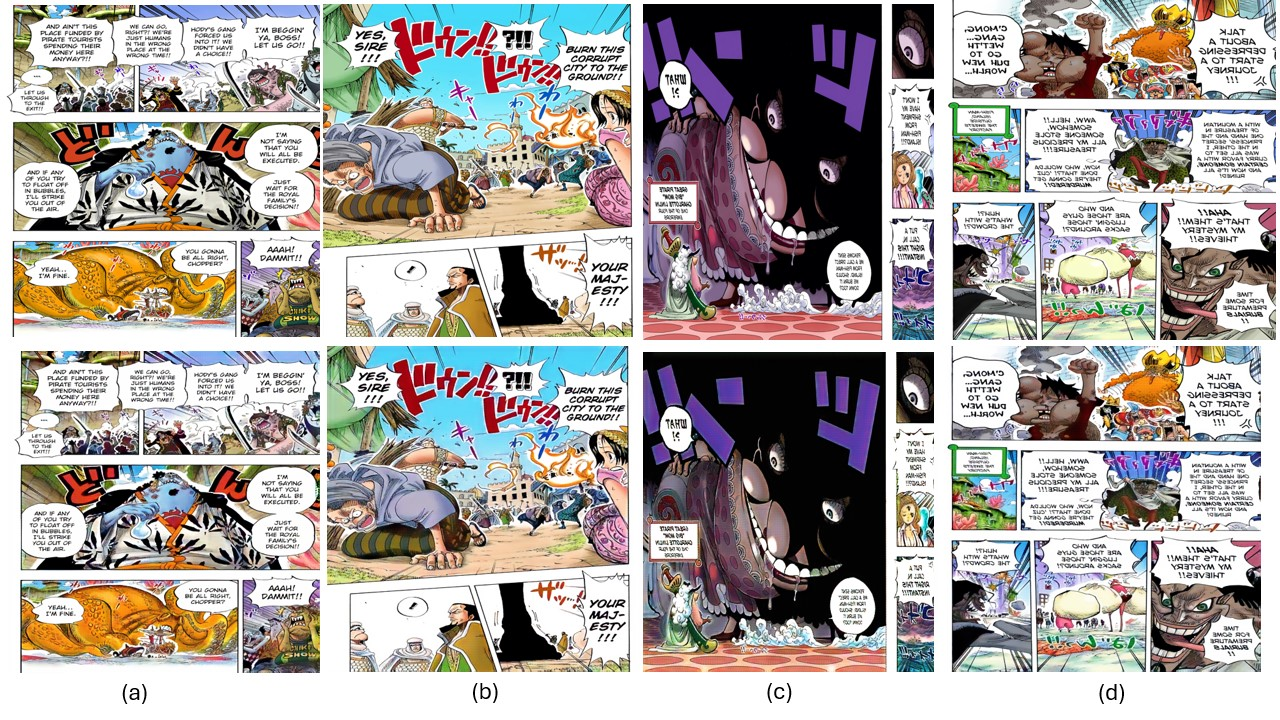
\includegraphics[height=0.4\textwidth]{img_psnr/perf_metrics.jpg}
    \caption{Real(top row) and Reconstructed colored (bottom row) images}
    \label{fig:comparision real and reconstructed}
\end{figure}


\begin{table} [htbp]
    \centering
    \begin{tabular}{|c|c|c|} \hline
         Image Pair Labels&  PSNR&  SSIM\\ \hline 
            a&  24.5019&  0.9404\\ \hline 
            b&  24.2575&  0.8277\\ \hline
            c& 24.8711& 0.9297\\\hline
            d& 23.8663& 0.9180\\\hline
            Average& 24.3742& 0.9039\\\hline
    \end{tabular}
    \label{tab:PSNR and SSIM table for real and reconstructed real images }
    \caption{PSNR and SSIM table for real and reconstructed real images }
\end{table}
